\chapter{Systemmodelle}


\section{Interaktionsverlauf}

Menüeinträge:

\begin{longtable}{|p{0.25\textwidth}|p{0.75\textwidth}|}
    \hline
    main menu & Das ist die erste Ansicht, die der Nutzer bekommt. Von hier aus erreicht er alle Bereiche des Programms.\\
    
    \hline
    
    creative & Von hier aus startet der Nutzer ein neues Spiel, mit einem einfachem Standardknoten, lädt einen Speicherstand oder startet das erstellen von neuen Herausforderungen (challenges).\\
    
    \hline
    
    challenge & Eine Übersicht, der vorhandenen Herausforderungen. Der Nutzer kann nach verschieden Kriterien suchen und sortieren lassen und in einer Vorschau weitere Informationen betrachten.\\

    \hline
    
    settings & Einstellungen an Grafik, Ton und Steuerung. Außerdem kann die persönliche Farbpalette angepasst werden.\\

    \hline
    
    credits & Zeigt Infos über die Mitwirkenden an dem Programm und über das Programm selber.\\

    \hline
    
   \end{longtable}
    
%	\begin{figure}[h]
%	  \centering
%	  \includesvg[svgpath=Systemmodelle/, width = 12.5cm]{menu}
%	  %\caption{...}
%	\end{figure}
	~\\
	Im Spiel kann der Nutzer auch die {\color{red} Einstellungen} erreichen. Die Menüeinträge in den unterschiedlichen Spielmodi können variieren.
\begin{longtable}{|p{0.25\textwidth}|p{0.75\textwidth}|}

	settings & Genau wie aus dem Hauptmenü.
    \hline
	save & Speichert den aktuellen Spielstand.
    \hline
	quit & Beendet das laufende Spiel.
    \hline
	render options & Bietet dem Nutzer verschiedene Möglichkeiten seinen Knoten zu rendern und zu exportieren.
\end{longtable}

	
\clearpage


\section{Benutzerinteraktionsmodelle}

	\begin{figure}[ht]
	  \centering
	  \includesvg[svgpath=Systemmodelle/, width = \textwidth]{inGame}
	  %\caption{...}
	\end{figure}
	
%	\begin{figure}[ht]
%		  \centering
%		  \includesvg[svgpath=Systemmodelle/, width = \textwidth]{Auswahl}
%		  %\caption{...}
%	\end{figure}
	
%	\begin{figure}[ht]
%		  \centering
%		  \includesvg[svgpath=Systemmodelle/, width = \textwidth]{ingamemenu}
%		  %\caption{...}
%	\end{figure}
	
	
%	\begin{figure}[ht]
%		  \centering
%		  \includesvg[svgpath=Systemmodelle/, width = \textwidth]{menu}
%		  %\caption{...}
%	\end{figure}
	
\clearpage
	
\subsection{Ungültige Züge}

	\begin{figure}[htb]
	  \centering
	  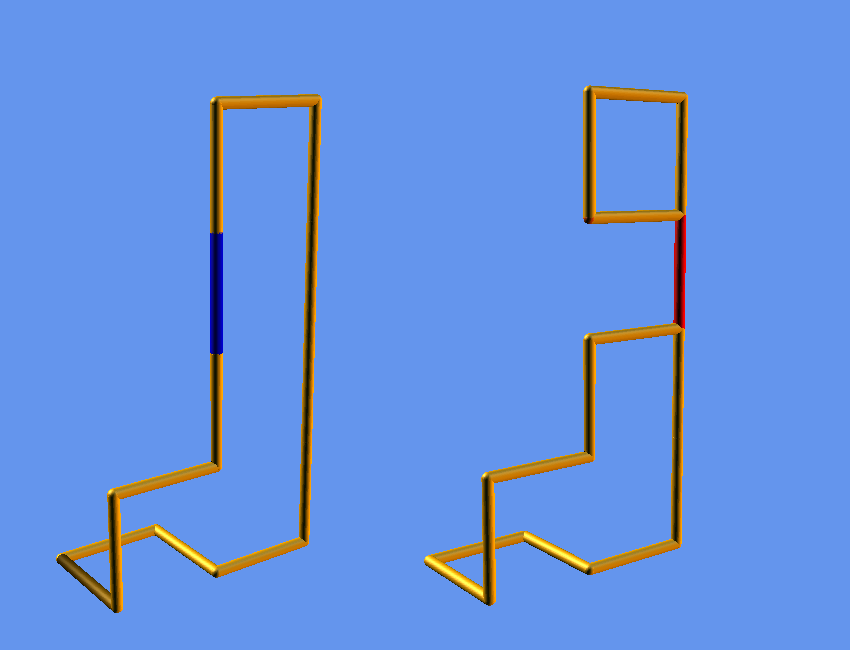
\includegraphics[width = \textwidth]{Systemmodelle/Ungueltiger_Zug.png}
	  \caption{...}
	  \label{fig:zug1}
	\end{figure}

Der Knoten auf der linken Seite \ref{fig:zug1} beschreibt eine gültige Spielsituation. Der Spieler wählt eine Kante (blaue Hervorhebung) aus, um einen weiteren Zug vorzunehmen.
Einem Spieler ist es nicht möglich, zwei parallele Kanten (hier: die Blaue und die Rote) zu einer Kante zu vereinen. Der Knoten soll immer aus einem geschlossenen Kreis von Kanten bestehen. Der Knoten auf der rechten Seite \ref{fig:zug1} ist daher eine ungültige Spielsituation.



	\begin{figure}[htb]
	  \centering
	  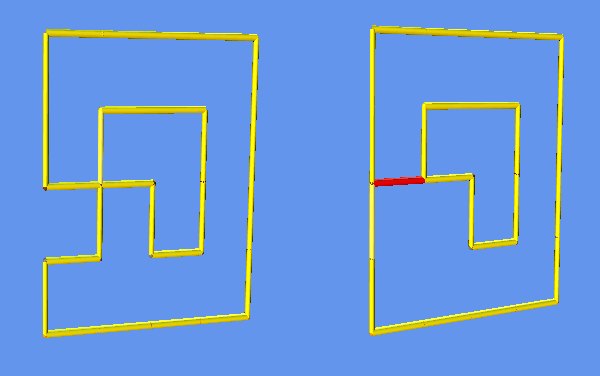
\includegraphics[width = \textwidth]{Systemmodelle/Ungueltiger_Zug2.png}
	  \caption{...}
	  \label{fig:zug2}
	\end{figure}

\clearpage

\section{Nutzerschnittstellen}

	\begin{figure}[ht]
	  \centering
	  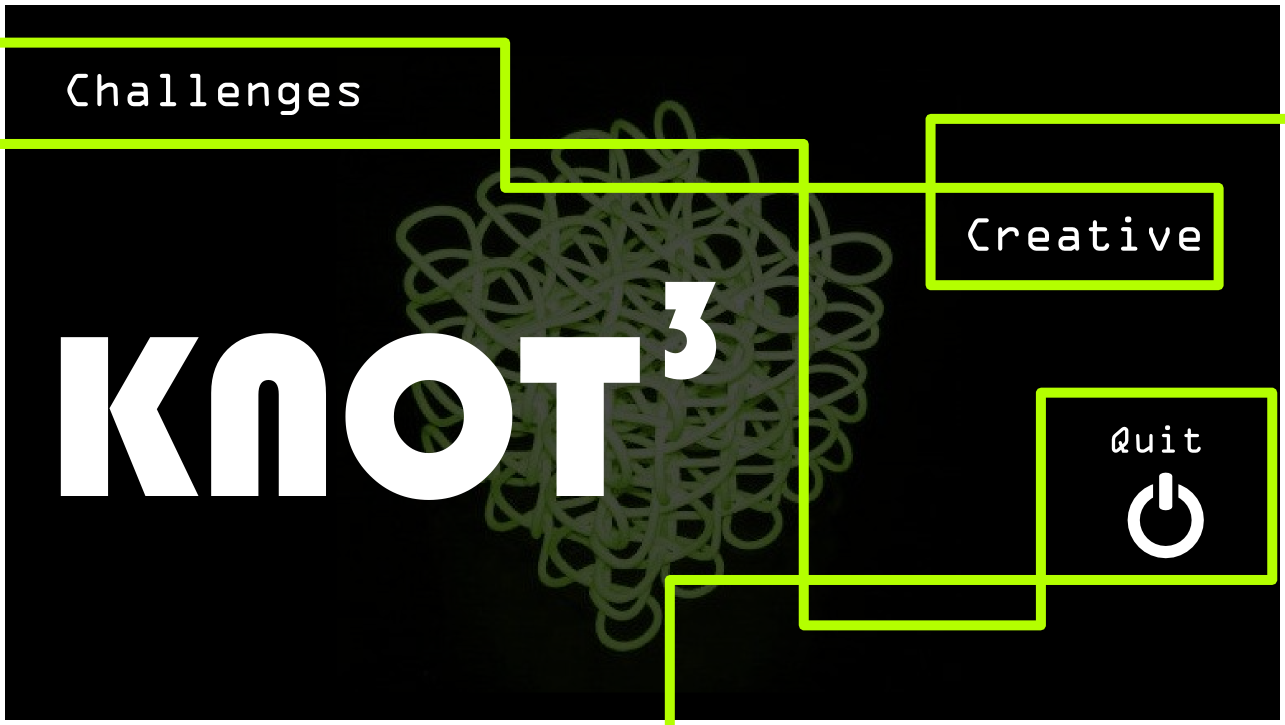
\includegraphics[width = \textwidth]{Systemmodelle/01_Knot3-mainscreen.png}
	  \caption{Hauptmenü}
	\end{figure}

	\begin{figure}[ht]
	  \centering
	  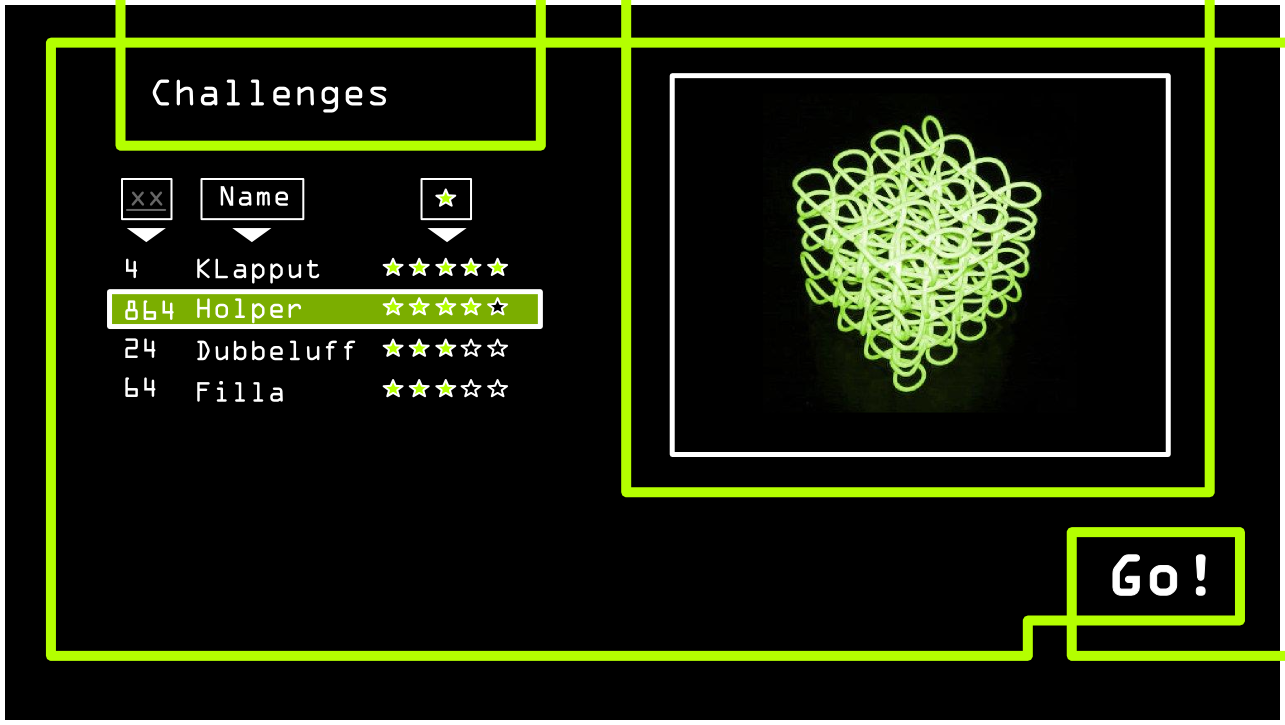
\includegraphics[width = \textwidth]{Systemmodelle/04_Knot3-select-Challenge.png}
	  \caption{Menü für Herausforderungen, mit Aussschnitt der Bestenliste}
	\end{figure}
	
	\begin{figure}[ht]
	  \centering
	  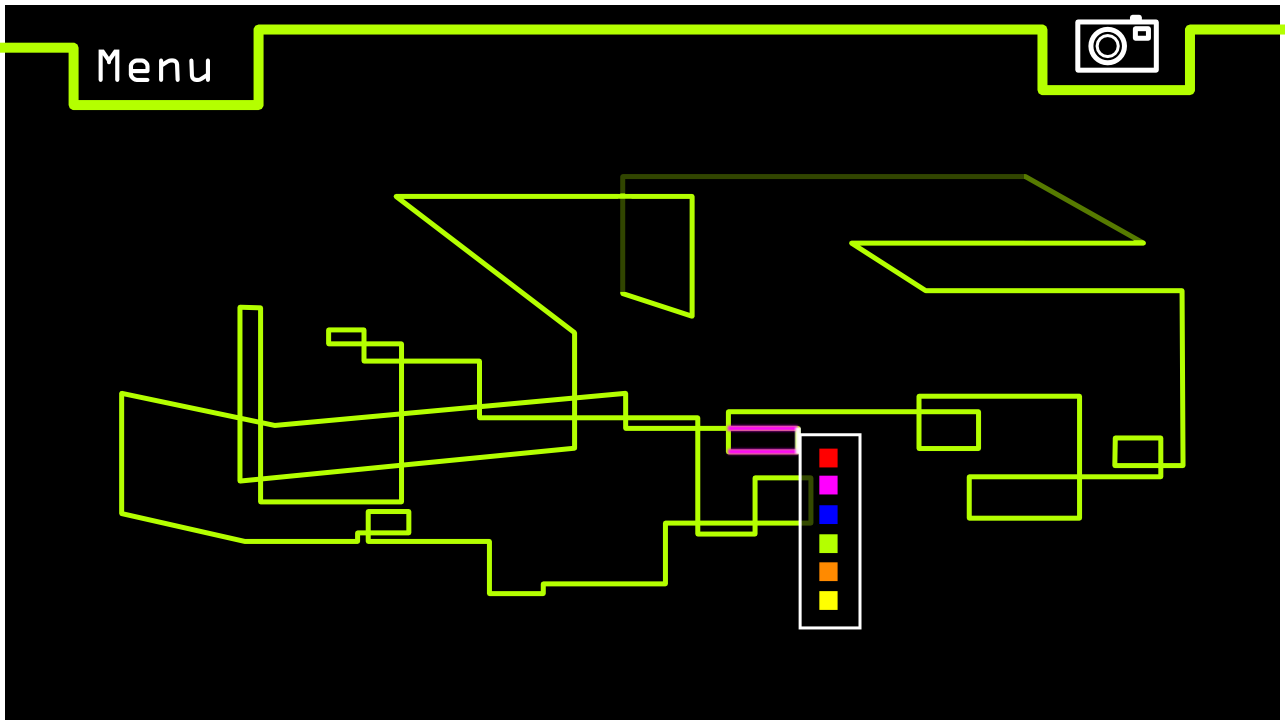
\includegraphics[width = \textwidth]{Systemmodelle/05_Knot3-Colour-select.png}
	  \caption{Creative: Kantenfärben}
	\end{figure}
	
	\begin{figure}[ht]
	  \centering
	  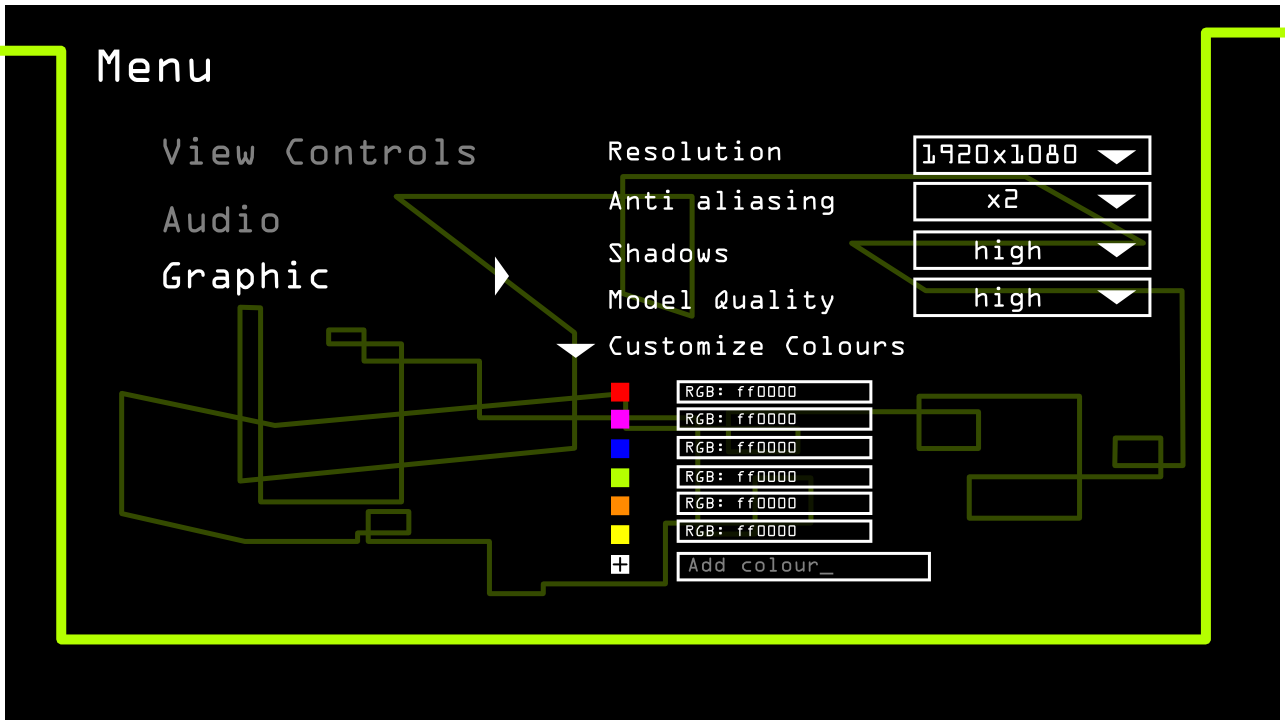
\includegraphics[width = \textwidth]{Systemmodelle/08_Knot3-menu-graphics.png}
	  \caption{Menü f. Grafikeinstellungen}
	\end{figure}

	
\clearpage
	
\section{Szenarien}
\begin{itemize}	
\item Der Spieler startet das Spiel und gelangt zum Hauptmenü. Dort wählt er den "creative" Modus und im darauf folgendem Menü das Erstellen eines neuen Knotens. Er gelangt in den Editor und beginnt dort den Knoten zu transformieren. Nach einigen transformationen öffnet er das Menü und speichert den Knoten. Danach fährt er mit der transformation fort. Zwischendurch ist er mit einigen Transformationsschritten unzufrieden und macht sie mir "undo" rückgängig. Nach einigen weiteren transformationen ruft er wieder das Menü auf, speichert und beendet daraufhin den Editor mit einem klick auf den Menüeintrag "quit". Daraufhin landet er wieder im Hauptmenü. Dort beendet er das Spiel.

\item Der Spieler startet das Spiel und gelangt zum Hauptmenü. Dort wählt er den "creative" Modus und danch "load" um einen alten Speicherstand zu laden. In der Auswahlliste wählt er den gewünschten Knoten aus und lädt diesen. Er landet im Editor. Dort betrachtet er Knoten ein Zeitlang von allen Seiten, indem er mit Tastatur und Maus die Kamera um den Knoten herum bewegt und beendet danach wieder den Editor.

\item  Der Spieler startet das Spiel und gelangt zum Hauptmenü. Dort wählt er den "challenge" Modus. Er sieht eine Liste mit allen verfügbaren Herausforderungen und einige Informationen zu diesen, dazu gehören die aktuellen Bestzeiten. Er sucht sich eine Herausforderung aus und Startet sie. Er landet im Editor mit einer zusätzlichen Ansicht für den Zielknoten. Er betrachtet diesen ausgiebig und beginnt danach mit der Transformation des vorgegebenen Knotens. Zum Zeitpunkt der ersten Transformation beginnt die Zeit zu laufen. Nach einigen Transformation stimmen die Knoten überein und die Zeit stoppt automatisch. Der Spieler war schnell und darf seinen Namen in die Bestenliste eintragen. Danach hat er die Möglichkeit die Herausforderung zu bewerten. Er gibt der Herausforderung eine gute Bewertung und landet danach wieder im Hauptmenü. Dort beendet er das Spiel.

\item Der Spieler startet das Spiel und gelangt zum Hauptmenü. Dort wählt er den "creative" Modus. Er möchte eine neue Herausforderung erstellen und wählt daher "new challenge". Danach wählt er zwei Knoten aus seinen Speicherständen aus. Einen für den Startknoten, einen als Zielknoten. Weiter unten gibt er der Herausforderung einen Namen und Speichert sie ab. Danach gelangt er in den Editor um als erster eine Zeit vorzulegen und die Herausfforderung zu bestreiten. Der Spieler beendet dei Herausforderung aber ohne sie abzuschließen. Er kann die Herausforderung noch bewerten und landet dann wieder im Hauptmenü. Dort beendet er das Spiel.
\end{itemize}

%	\begin{figure}[ht]
%	  \centering
%	  \includesvg[svgpath=Systemmodelle/, width = \textwidth]{Anwendungsfall}
%	  %\caption{...}
%	\end{figure}


